\documentclass[12pt]{article}
%%%%%%%%%%%%%%%%%%%%%%%%%%%%%%%%%%%%%%%%%%%%%%%%%%%%%
%%%%%%%%%%%  MATH  %%%%%%%%%%%%%%%%%%%%%%%%%%%%%%%%%%
\usepackage{amsmath,amsthm,amssymb} %math
\usepackage{xfrac} %sfrac
\usepackage{faktor} %better than sfrac
\usepackage{dutchcal} %some font for mathcal
\usepackage{array} %for newcoltype
\newlength\mylen
\newcolumntype{R}{>{\hfill$}p{\mylen}<{$}}
\settowidth\mylen{$-1$}
%\everymath{\displaystyle} %to show every math big
%%%%%%%%%%%%%%%%%%%%%%%%%%%%%%%%%%%%%%%%%%%%%%%%%%%%%
%%%%%%%%%%%  OTHER PACKAGES  %%%%%%%%%%%%%%%%%%%%%%%%
\usepackage[utf8]{inputenc} %encoding
\usepackage{hyperref} %hyperlinks
\usepackage{geometry} %page size and margins
\usepackage{makeidx} %indexing
\usepackage{graphicx} %inclusion of graphics
\usepackage{wrapfig} %wrap text around figures
\usepackage{xstring} %manipulate strings
\usepackage[dvipsnames]{xcolor} %colors !conflicts with beamer!
%%%%%%%%%%%%%%%%%%%%%%%%%%%%%%%%%%%%%%%%%%%%%%%%%%%%%
%%%%%%%%%%%  TIKZ 4 LIFE  %%%%%%%%%%%%%%%%%%%%%%%%%%%
\usepackage{tikz}
\usetikzlibrary{cd} %commutative diagrams
\usetikzlibrary{decorations} %curved lines
\usetikzlibrary{positioning} %coordinates positioning
%\usetikzlibrary{replacements} %right=of nodename
\usetikzlibrary{3d,calc} %coordinate calculations & 3d
%%%%%%%%%%%%%%%%%%%%%%%%%%%%%%%%%%%%%%%%%%%%%%%%%%%%%
%%%%%%%%%%%  CUSTOMIZE THE LOOKS  %%%%%%%%%%%%%%%%%%%
\geometry{headheight=15pt}
%\setlength\parskip{\baselineskip} %space between paragraphs
\setlength\parindent{0pt} %no indentation
%%%%%%%%%%%%%%%%%%%%%%%%%%%%%%%%%%%%%%%%%%%%%%%%%%%%%
%%%%%%%%%%%  ENUMERATE / ITEMIZE  %%%%%%%%%%%%%%%%%%%
\usepackage{enumerate} %enumerate/itemize (has to be first)
\usepackage{enumitem} %customize enumerate/itemize
% \setlist{nolistsep} %<=> [nosep] <=> Kills vert sep <=> ![listsep]
\newenvironment{n_enum}{\begin{enumerate}[label=(\arabic{*})]}{\end{enumerate}} %1,2,3,...
\newenvironment{i_enum}{\begin{enumerate}[label=(\roman{*})]}{\end{enumerate}} %i,ii,iii,...
\newenvironment{a_enum}{\begin{enumerate}[label=(\alph{*})]}{\end{enumerate}} %a,b,c,...
\newenvironment{b_item}{\begin{itemize}}{\end{itemize}} %bullets
%%%%%%%%%%%%%%%%%%%%%%%%%%%%%%%%%%%%%%%%%%%%%%%%%%%%%
%%%%%%%%%%%  MATH NOTATIONS  %%%%%%%%%%%%%%%%%%%%%%%%
\newenvironment{eqarray}{\begin{array}{>{\displaystyle}r>{\displaystyle}c>{\displaystyle}l}}{\end{array}}
\newcommand\Hom{\mathrm{Hom}}
\newcommand\NHom{\mathrm{NHom}}
\newcommand\ChRmod{Ch($R$-mod)}
\newcommand\ChZmod{Ch($\mathbb{Z}$-mod)}
\newcommand\KRmod{$\mathcal{K}$($R$-mod)}
\newcommand\Csing[1]{C^{\mathrm{sing}}\left(#1\right)}
\newcommand\Dtop[1]{\Delta^{\mathrm{top}}\left(#1\right)}
\newcommand\Tor{\mathrm{Tor}}
\newcommand\Ext{\mathrm{Ext}}
\newcommand\Mod{\mathrm{Mod}}
\newcommand\Ab{\mathrm{Ab}}
\newcommand\map{\mathrm{map }}
\newcommand\im{\mathrm{im\ }}
\newcommand\tensor{\otimes}
%\newcommand\ker{\mathrm{ker}}
\newcommand\coim{\mathrm{coim\ }}
\newcommand\coker{\mathrm{coker\ }}
\newcommand\cupdot{\mathbin{\mathaccent\cdot\cup}}
\newcommand\rank{\mathrm{rank}}
\newcommand\val{\mathrm{val}}
%%%%%%%%%%%%%%%%%%%%%%%%%%%%%%%%%%%%%%%%%%%%%%%%%%%%%
%%%%%%%%%%%  OTHER NOTATIONS  %%%%%%%%%%%%%%%%%%%%%%%
\newcommand\ul[1]{\emph{#1}}
\newcommand\nospace{\hspace*{-0.5em}}
\newcommand\HRule{\rule{\linewidth}{0.1mm}}
%%%%%%%%%%%%%%%%%%%%%%%%%%%%%%%%%%%%%%%%%%%%%%%%%%%%%
%%%%%%%%%%%  BEGIN DOCUMENT  %%%%%%%%%%%%%%%%%%%%%%%%
\begin{document}
\begin{center}
{\bf Mathematical Aspects of Public Transportation Networks}\\
Problem Set 10
\end{center}
So 2018 \hfill Dimitrios Bogiokas - BMS\\
\phantom{X}\hfill FU ID: 5048996\\
\HRule\\
{\bf Exercise 1} \begin{a_enum}
\item Let $l_e$ be the trivial path containing only the edge $e$, for every $e\in E$. Then the vector $x\in\{0,1\}^{\mathcal{L}}$, with:
$$x_l=\left\{\begin{array}{lcl}
1&,&\exists e\in E:\ l=l_e\\
0&,&\text{else}\\
\end{array}\right.$$
is a solution to the $k$-line pool problem, if $k\geq|E|$. Indeed:
$$\sum_{l\in\mathcal{L}}x_l=|E|\leq k$$
Moreover, choose the vector $f\in(\mathbb{N}_0)^{\mathcal{L}}$ to be:
$$f_l=\left\{\begin{array}{lcl}
f_e^{\min}&,&\exists e\in E:\ l=l_e\\
0&,&\text{else}\\
\end{array}\right.$$
obviously satisfying $f_l\leq Fx_l$ for all $l\in\mathcal{L}$.
Then, for every $e\in E$, we have:
$$\sum_{l\in\mathcal{L}_e}f_l=f_{l_e}=f_e^{\min}\in[f_e^{\min},f_e^{\max}]$$
\item Let $G=(V,E)$ be a directed graph. Define then the undirected graph $\tilde G=(\tilde V,\tilde E)$, with vertices:
$$\tilde V:=\bigcup_{v\in V}\{v^i,v^o\}$$
and edges:
$$\tilde E:=\bigcup_{v\in V}\big\{\{v^i,v^o\}\big\}\cup\bigcup_{(u,v)\in E}\big\{\{u^o,v^i\}\big\}$$
Also let $k=1$ and for every $e\in\tilde E$, let $f_e^{\max}=1$ and:
$$f_e^{\min}=\left\{\begin{array}{lcl}
1&,&e=\{v^i,v^o\}\\
0&,&e=\{u^o,v^i\}\\
\end{array}\right.$$

Obviously we have then also $F=1$. Then, the $1$-line pool generation problem on $\tilde G$, with this frequency function has a solution if and only if $G$ has a directed Hamilton path. Indeed:

$(\Leftarrow)$ Let $P=(v_1,v_2,\ldots,v_n)$ be a directed Hamilton path on $G$. Define then:
$$\tilde P:=(v_1^i,v_1^o,v_2^i,v_2^o,\ldots,v_n^i,v_n^o)$$
to be a walk in $\tilde G$. This is indeed a walk, since the edges $\{v_j^i,v_j^o\}$ are indeed elements of $\tilde E$, for every $j\in[n]$ and also the edges $\{v_j^o,v_{j+1}^i\}$ are also elements in $\tilde E$, for every $j\in[n-1]$, since $(v_j,v_{j+1})\in E$. Moreover, $\tilde P$ is vertex-distinct and thus a path, since $P$ was vertex-distinct.
Let now $x_{\tilde P}=f_{\tilde P}=1$ and $x_l=f_l=0$, for all other paths $l$. Then, obviously $f_l=Fx_l$, for every $l\in\tilde{\mathcal{L}}$, path in $\tilde G$, and $\sum_{l\in\tilde{\mathcal{L}}}x_l=1=k$. Moreover, let $e\in\tilde E$. Then, we have:
\begin{b_item}
\item If $e=\{v^i,v^o\}$ for some $v\in V$, we have that $P$ goes through $v$ (since it is a Hamilton path) and thus $v=v_j$ for some index $j$. This means that $e$ is an edge of $\tilde P$, which gives:
$$\sum_{l\in\tilde{\mathcal{L}}_e}f_l=f_{\tilde P}=1=f_e^{\min}=f_e^{\max}$$
\item If $e=\{u^o,v^i\}$ for some $(u,v)\in E$, we have that:
$$f_e^{\min}=0\leq\sum_{l\in\tilde{\mathcal{L}}_e}f_l\leq f_{\tilde P}=1=f_e^{\max}$$
where the second inequality depends on $e$ being an edge of $\tilde{P}$ or not.
\end{b_item}

$(\Rightarrow)$ For the inverse, consider $x\in\{0,1\}^{\tilde{\mathcal{L}}}$ be a solution to this $1$-line pool generation problem on $\tilde G$. Since
$$\sum_{l\in\tilde{\mathcal{L}}}x_l\leq 1$$
we have that either $x_l=0$ for every path $l\in\tilde{\mathcal{L}}$, or there exists a path $L\in\tilde{\mathcal{L}}$ with $x_L=1$ and $x_l=0$ otherwise. In the first case, we also get that $f_l\leq Fx_l=0$. Let $v\in V$ be any vertex. Then for the edge $e=\{v^i,v^o\}\in\tilde E$, we get:
$$\sum_{l\in\tilde{\mathcal{L}}_e}f_l=0<1=f_e^{\min}$$
This means, that this cannot be true and leaves us only with the latter case. We first prove that this path $L$ is a Hamilton path in $\tilde G$. Indeed, let $v\in V$. Then, for the edge $e=\{v^i,v^o\}\in\tilde E$ we have:
$$f_e^{\min}\leq\sum_{l\in\tilde{\mathcal{L}}_e}f_l\leq f_L=1=f_e^{\min}$$
where the second inequality is an equality only if $L\in\tilde{\mathcal{L}}_e$. Since in the expression above every inequality is an equality, we have that $e$ is an edge in the path $L$. In particular, both $v^i$ and $v^o$ are vertices in this path. Next notice that $\tilde G$ is a bipartite graph (colour every vertex of the form $v^i$ red and everyone of the form $v^o$ blue), which means in particular, that the vertices of the path $L$ alternate between these two forms, if one moves along the path. Since the two parts of $\tilde{G}$ have the same amount of vertices, namely $n=|V|$, we know that $L$ starts with some vertex of the form $v^i$ and ends with one of the form $u^o$, or the other way around. Without loss of generality, we will assume that $L$ is of the former type. Indeed, if $L$ is of the latter type, just reversing the traversing direction of $L$, gives us a new path of the former type, satisfying the same assumptions.

Since all edges of the form $\{v^i,v^o\}$ are edges of $L$, we make the following two observations:
\begin{b_item} \item It can never have the case that $(\ldots,u^o,v^i,w^o,\ldots)$ is a piece of the path for $u\neq v\neq w$ (Because otherwise $v^i$ would have degree at least $3$ in the path). Thus, at least one of $u,w$ are the same as $v$ (in fact exactly one).
\item It cannot be the case that $(v^i,u^o,\ldots)$ is the start of the path for $v\neq u$ (Because otherwise $v^i$ would have degree at least $2$ in the path, but it is an endpoint).
\end{b_item}
These facts mean, that $L$ has the following form:
$$(v_1^i,v_1^o,v_2^i,v_2^o,\ldots,v_n^i,v_n^o)$$
for some ordering $v_1,v_2,\ldots,v_n$ of the vertices in $V$.
Define then $\bar L$ in $G$ to be the walk $(v_1,v_2,\ldots,v_n)$. This is indeed a directed walk, since $\{v_j^o,v_{j+1}^i\}$ is in $\tilde E$ iff $(v_j,v_{j+1})$ is in $E$. Then we can easily see that $\bar L$ is in fact a path, because $L$ was already vertex-distinct, which gives in particular that $v_i\neq v_j$ for every $i\neq j$. So, we proved that $\bar L$ is a Hamiltonian path in $G$.

For completeness reasons, it should also be mentioned that this reduction from the directed Hamiltonian path problem to the $1$-line generation pool problem is computable in polynomial time. Indeed, on any graph input we need linear time to define the new graph and the capacity functions.
\end{a_enum}
{\bf Exercise 2} The Steiner connectivity problem is finding a vector $x\in\{0,1\}^{\mathcal{P}}$, which minimizes
$$\sum_{P\in\mathcal{P}}x_Pc_P$$
under the constrains that
$$T\subseteq\bigcup_{\underset{x_P=1}{P\in\mathcal{P}}}V(P)$$
and that
$$\bigcup_{\underset{x_P=1}{P\in\mathcal{P}}}P\text{ is connected}$$
We will prove that a vector $x\in\{0,1\}^{\mathcal{P}}$ solves the Steiner connectivity problem iff it is a solution for the given integer program, up to zero-weight paths. This means that there might exist some $x\in\{0,1\}^{\mathcal{P}}$ solving the given integer program and not solving the Steiner connectivity problem, but we will prove that in this case there exists some $x'\leq x$, such that
$$0=x_P'<x_P=1\ \ \Rightarrow\ \ c_P=0$$Since the quantity that should be minimized is the same, it suffices to prove that the above mentioned constrains are satisfied by some $x$ (up to zero-valued paths), iff $x$ satisfies the constrain:
$$\sum_{P\in\mathcal{P}(W)}x_P\geq1\qquad\forall W\subseteq V,\ \emptyset\neq W\cap T\neq T$$

$(\Rightarrow)$ Let $x\in\{0,1\}$ satisfying the two constrains of Steiner connectivity problem and let $W\subseteq V$, with $\emptyset\neq W\cap T\neq T$. Since $W\cap T\neq T$, there exists some terminal $t\not\in W$ and since $W\cap T\neq\emptyset$, there exists some terminal $t'\in W$. Due to the first constraint, $t,t'\in\bigcup_{\underset{x_P=1}{P\in\mathcal{P}}}V(P)$, which in particular means that there exist nodes of the path collection both in $W$ and not in $W$. Since the union of paths is connected in $G$, there exists some path $P$ with some vertex in $W$ and some not in $W$. Thus, this path $P$ has an edge $e$, with $|e\cap W|=1$, i.e. $P\in\mathcal{P}(W)$.

$(\Leftarrow)$ For the inverse, let $x\in\{0,1\}$ satisfying the constrain of the integer program. And let $t\in T$. For the set $W=\{t\}$ apply the integer-programing constrain, which gives us exactly that there exists some path $P$, with $x_P=1$ passing through $t$, i.e. $t\in\bigcup_{\underset{x_P=1}{P\in\mathcal{P}}}V(P)$, giving us the inclusion $T\subseteq\bigcup_{\underset{x_P=1}{P\in\mathcal{P}}}V(P)$. Let
$$C\subseteq\bigcup_{\underset{x_P=1}{P\in\mathcal{P}}}P$$
be a connected component of the union of paths, containing at least one terminal $t\in T$. If there exists some $t'\in T\setminus C$, then for $W=C$, using the integer program constrain, we get some path $P\in\mathcal{P}(C)$ with $x_P=1$ having vertices both in $C$ and outside $C$, wich contradicts the choice of $C$. Thus, $T\subseteq C$. Let $x'\in\{0,1\}^{\mathcal{P}}$, with
$$x_P'=\left\{\begin{array}{lcl}x_P&,&P\subseteq C\\0&,&\text{otherwise}\\\end{array}\right.$$
Then, obviously $x'\leq  x$ and if any path is satisfying $0=x_P'<x_P=0$, then $P$ cannot include any terminals in its vertices, thus ommiting $P$ also gives a valid solution to the linear program. In fact ommiting $P$ gives a strictly better solution, w.r.t. the minimization, unless $c_P=0$, which is exactly the case described above.

{\bf Exercise 3} \begin{a_enum}
\item Let $G$ be the given graph and $G^{c}$ be its metric closure, w.r.t. the given edge costs $c$. For this we used the Floyd-Warshall algorithm in the C++ program you can find attached. This returned the following distance matrix:
$$\begin{array}{ll|r|r|r|r|r|r|r|}
&&A&B&C&D&E&F&G\\[0.5em]\hline
A&&0&25&31&15&12&20&21\\\hline
B&&25&0&15&32&13&10&20\\\hline
C&&31&15&0&22&19&20&10\\\hline
D&&15&32&22&0&21&22&12\\\hline
E&&12&13&19&21&0&8&9\\\hline
F&&20&10&20&22&8&0&10\\\hline
G&&21&20&10&12&9&10&0\\\hline
\end{array}$$
which is of course symmetric. Moreover, we notice that the smallest distance between two vertices joined by an edge is the cost of this edge.

Then, we know that it suffices to find the cost of a Minimum Weight Spanning Tree in $G^c$ and one in $G^c\setminus v_E$ and compare their costs. Theoretically after that, we should compute the induced trees in $G$, but the program so happens to output MWSTs with edges also existing in the original graph (with the same cost, as we just mentioned). Thus, the two spanning trees of interest are:
\begin{center}
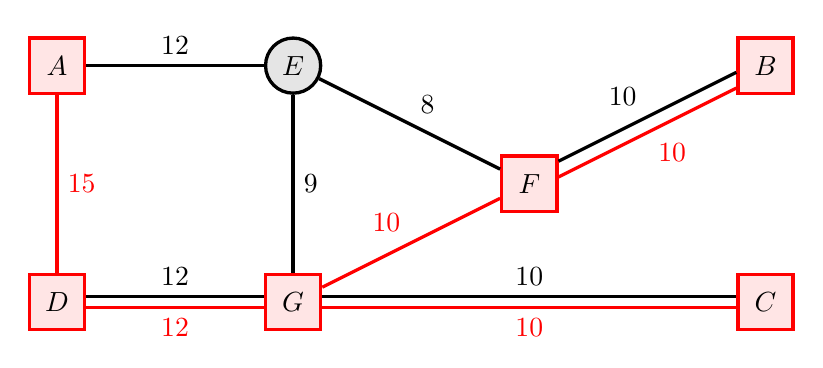
\begin{tikzpicture}[scale = 3,
node/.style = {minimum size=7mm, very thick},
terminal/.style = {node, rectangle, draw=red, fill=red!10},
simple/.style = {node, circle, draw=black, fill=black!10},
mwst/.style = {very thick},
mwstRed/.style = {mwst, draw=red},
labelRed/.style = {red},
mwstBlack/.style = {mwst, draw=black},
labelBlack/.style = {black}]
\def\bit{.7mm};
\def\bitsqrttwo{1mm};
\node[terminal] (A) at (0,1) {$A$};
\node[terminal] (B) at (3,1) {$B$};
\node[terminal] (C) at (3,0) {$C$};
\node[terminal] (D) at (0,0) {$D$};
\node[simple] (E) at (1,1) {$E$};
\node[terminal] (F) at (2,.5) {$F$};
\node[terminal] (G) at (1,0) {$G$};

\draw[mwstBlack] (A) to node[labelBlack, auto] {$12$} (E);
\draw[mwstBlack] (E) to node[labelBlack, auto] {$8$} (F);
\draw[mwstBlack] (E) to node[labelBlack, auto] {$9$} (G);
\draw[mwstBlack, transform canvas={yshift=\bit}] (G) to node[labelBlack, auto] {$10$} (C);
\draw[mwstBlack, transform canvas={yshift=\bitsqrttwo}] (F) to node[labelBlack, auto] {$10$} (B);
\draw[mwstBlack, transform canvas={yshift=\bit}] (G) to node[labelBlack, auto,swap] {$12$} (D);

\draw[mwstRed] (A) to node[labelRed, auto] {$15$} (D);
\draw[mwstRed, transform canvas={yshift=-\bit}] (D) to node[labelRed, auto,swap] {$12$} (G);
\draw[mwstRed, transform canvas={yshift=-\bit}] (G) to node[labelRed, auto,swap] {$10$} (C);
\draw[mwstRed] (G) to node[labelRed, auto] {$10$} (F);
\draw[mwstRed, transform canvas={yshift=-\bitsqrttwo}] (F) to node[labelRed, auto,swap] {$10$} (B);

\end{tikzpicture}
\end{center}
with red colour a MWST of cost $57$ in $G^c\setminus v_E$ and with black a MWST of cost $61$ in $G^c$. 

Of these two, the red one has less cost and thus this is a Steiner tree of $G$ of minimum cost.
\item For this we used a C++ program to generate an MIP minimizing the sum of the frequences each line is used. The two directions of each line $l$ were regarded as different lines, numbered as $l$ and $l+7$. Unfortunately, optimal solutions of this MIP did not in general avoid loops of imaginary passengers, traveling on empty spaces in the lines used for solving the program. I removed one such loop by hand from the SCIP solution, to get the following valid line plan:

\begin{center}
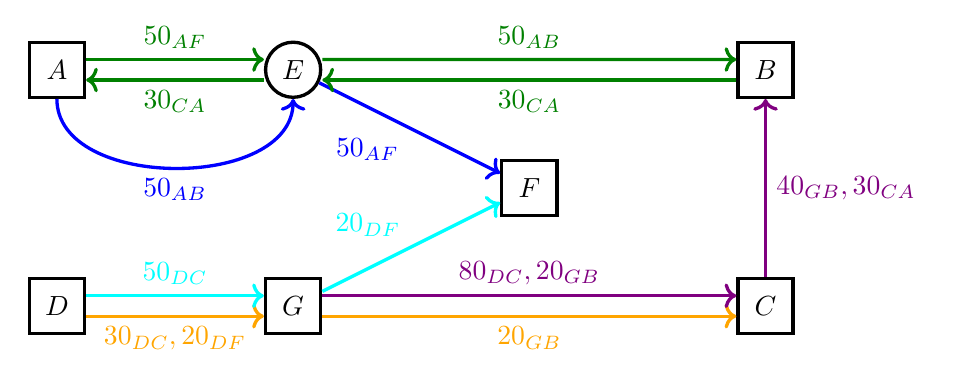
\begin{tikzpicture}[scale = 3,
node/.style = {minimum size=7mm, very thick, draw=black},
terminal/.style = {node, rectangle},
simple/.style = {node, circle},
edge/.style = {very thick,->},
edge2/.style = {edge, draw=Green},
label2/.style = {Green},
edge3/.style = {edge, draw=Blue},
label3/.style = {Blue},
edge4/.style = {edge, draw=Orange},
label4/.style = {Orange},
edge6/.style = {edge, draw=Purple},
label6/.style = {Purple},
edge7/.style = {edge, draw=Cyan},
label7/.style = {Cyan}]
\def\bit{1.3mm};
\node[terminal] (A) at (0,1) {$A$};
\node[terminal] (B) at (3,1) {$B$};
\node[terminal] (C) at (3,0) {$C$};
\node[terminal] (D) at (0,0) {$D$};
\node[simple] (E) at (1,1) {$E$};
\node[terminal] (F) at (2,.5) {$F$};
\node[terminal] (G) at (1,0) {$G$};

\draw[edge2,transform canvas={yshift=\bit}] (A) to node[label2, auto] {$50_{AF}$} (E);
\draw[edge2,transform canvas={yshift=\bit}] (E) to node[label2, auto] {$50_{AB}$} (B);
\draw[edge3] (A) to [out=270,in=270] node[label3, auto, swap] {$50_{AB}$} (E);
\draw[edge3] (E) to node[label3, auto, swap] {$50_{AF}$} (F);
\draw[edge4,transform canvas={yshift=-\bit}] (D) to node[label4, auto, swap] {$30_{DC},20_{DF}$} (G);
\draw[edge4,transform canvas={yshift=-\bit}] (G) to node[label4, auto, swap] {$20_{GB}$} (C);
\draw[edge7,transform canvas={yshift=\bit}] (D) to node[label7, auto] {$50_{DC}$} (G);
\draw[edge7] (G) to node[label7, auto] {$20_{DF}$} (F);
\draw[edge2,transform canvas={yshift=-\bit}] (B) to node[label2, auto] {$30_{CA}$} (E);
\draw[edge2,transform canvas={yshift=-\bit}] (E) to node[label2, auto] {$30_{CA}$} (A);
\draw[edge6,transform canvas={yshift=\bit}] (G) to node[label6, auto] {$80_{DC},20_{GB}$} (C);
\draw[edge6] (C) to node[label6, auto, swap] {$40_{GB},30_{CA}$} (B);
\end{tikzpicture}
\end{center}
where, the labels are the number of people traveling on each line and the subscripts denote the demands these people satisfy. Also with different colours we denote different lines:
\begin{center}
\begin{tabular}{lll}
Line 2&AEB&Green\\\hline
Line 3&AEF&Blue\\\hline
Line 4&DGC&Orange\\\hline
Line 6&BCGF&Purple\\\hline
Line 7&DGF&Cyan\\
\end{tabular}
\end{center}
In the solution above, we use Line 2 twice, Line 3 once, Line 4 once, Line 6 twice and Line 7 once. This makes a total of $7$ lines used.
\end{a_enum}
\end{document}
